\begin{frame}{}
    \LARGE NLP: \textbf{Transformers}
\end{frame}

\begin{frame}[allowframebreaks]{Transformers: Overview}
    \begin{figure}
        \centering
        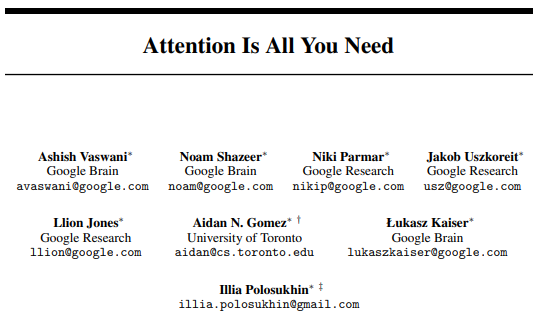
\includegraphics[width=\linewidth, height=0.9\textheight,keepaspectratio]{images/nlp/transformers-paper.png}
    \end{figure}
    \framebreak

    \begin{columns}[T,onlytextwidth]
        \begin{column}{0.6\textwidth}
            \textbf{Key Features:}
            \begin{itemize}
                \setlength{\itemsep}{1em}
                \item Transformers revolutionized NLP by using self-attention mechanisms.
                \item They process entire sequences simultaneously, unlike RNNs.
                \item Key components:
                \begin{itemize}
                    \item Multi-head self-attention
                    \item Positional encoding
                    \item Feed-forward neural networks
                \end{itemize}
                \item Transformers can handle long-range dependencies effectively.
            \end{itemize}
        \end{column}
        \begin{column}{0.5\textwidth}
            \centering
            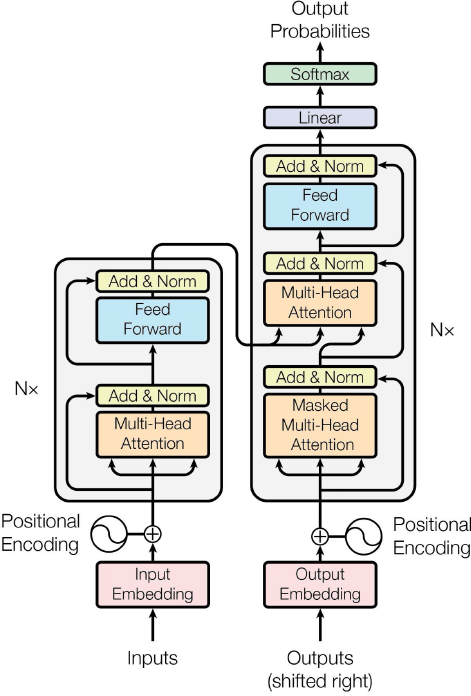
\includegraphics[width=\linewidth, height=0.9\textheight,keepaspectratio]{images/nlp/transformer-architecture.png}
        \end{column}
    \end{columns}
\end{frame}

\begin{frame}[allowframebreaks]{Machine Translation with Transformers}

    \begin{columns}
        \begin{column}{0.6\textwidth}
            \centering
            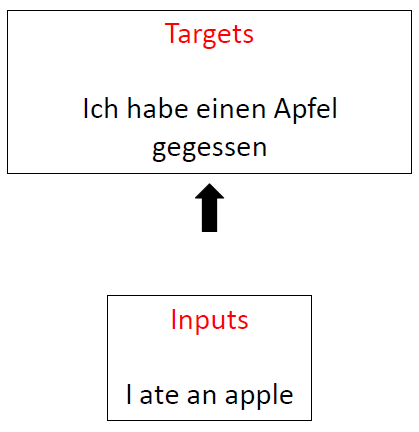
\includegraphics[width=\textwidth, height=0.9\textheight,keepaspectratio]{images/nlp/machine-translation.png}
        \end{column}
        \begin{column}{0.5\textwidth}
            \centering
            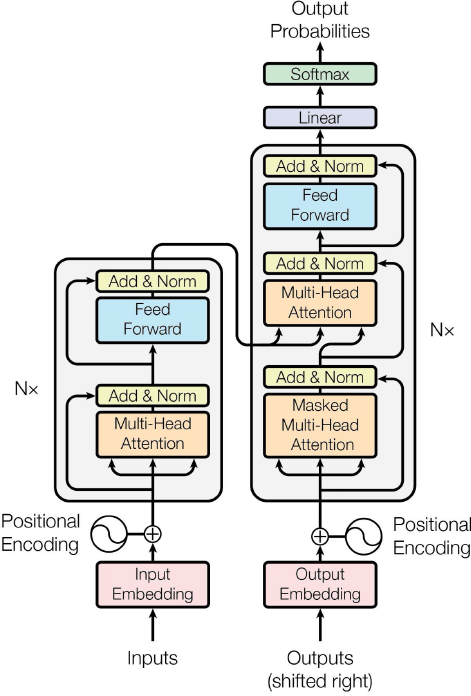
\includegraphics[width=\linewidth, height=0.9\textheight,keepaspectratio]{images/nlp/transformer-architecture.png}
        \end{column}
    \end{columns}
\end{frame}

\begin{frame}{Input Embeddings}
    \begin{figure}
        \centering
        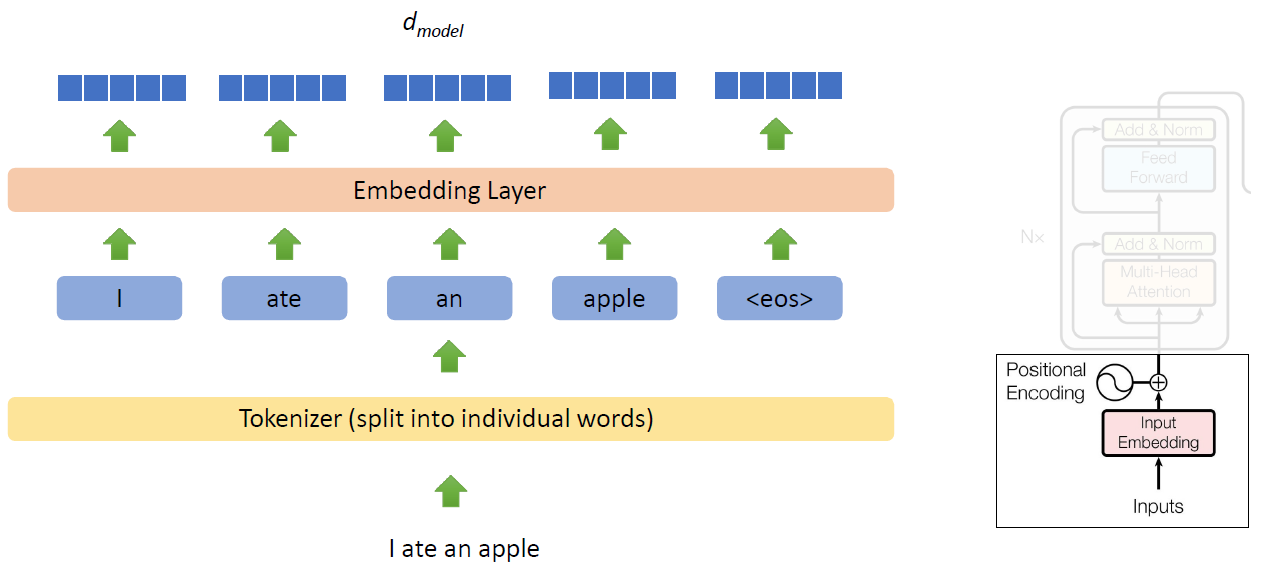
\includegraphics[width=\linewidth, height=0.9\textheight,keepaspectratio]{images/nlp/input-embeddings.png}
    \end{figure}

    \textbf{Input embeddings} are dense vector representations of input tokens, allowing the model to understand semantic relationships.
\end{frame}

\begin{frame}[allowframebreaks]{Position Encodings}
    \textbf{Position encodings} are added to input embeddings to provide information about the position of tokens in the sequence, enabling the model to capture order and structure.

    \framebreak
    \begin{figure}
        \centering
        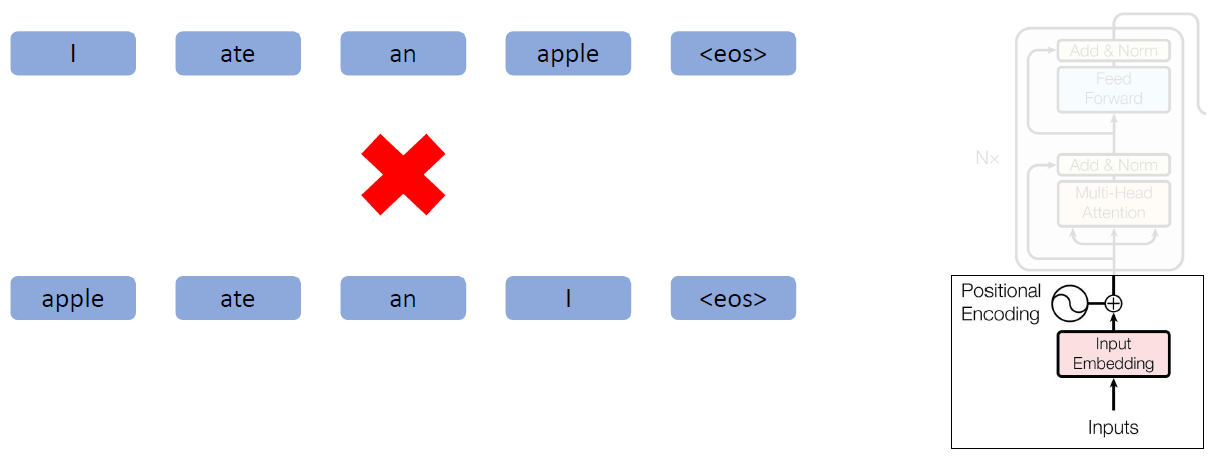
\includegraphics[width=\linewidth, height=0.9\textheight,keepaspectratio]{images/nlp/position-encodings.png}
    \end{figure}

    \framebreak
    \begin{figure}
        \centering
        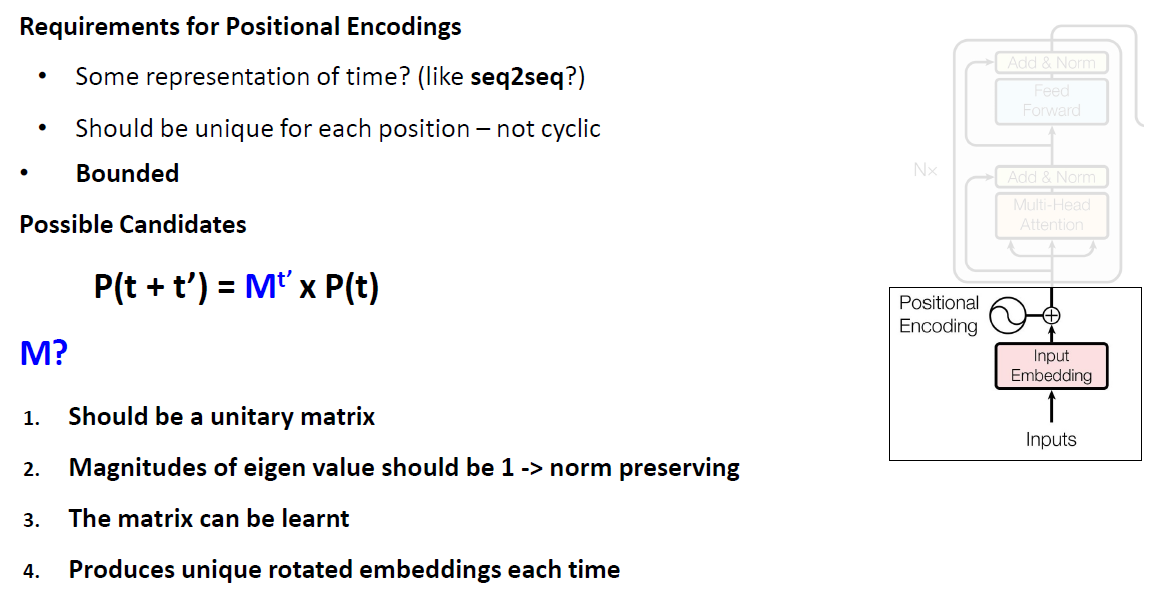
\includegraphics[width=\linewidth, height=0.9\textheight,keepaspectratio]{images/nlp/position-encodings-2.png}
    \end{figure}

    \framebreak
    \begin{figure}
        \centering
        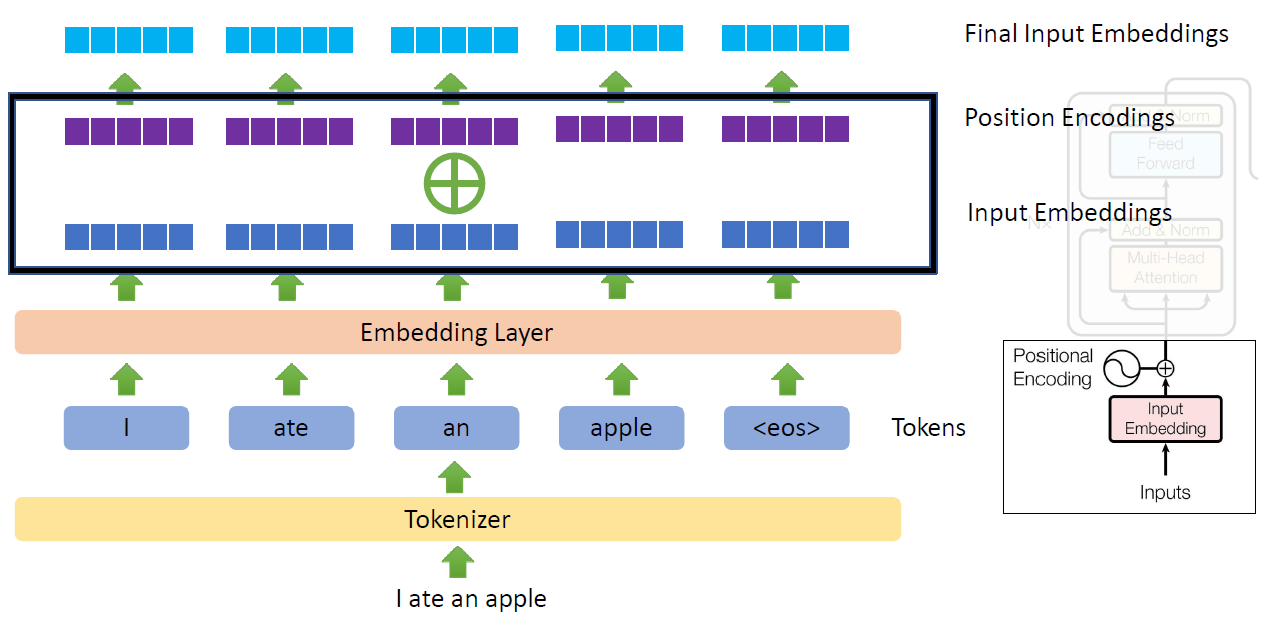
\includegraphics[width=1.05\linewidth, height=0.9\textheight,keepaspectratio]{images/nlp/position-encodings-3.png}
    \end{figure}
\end{frame}

\begin{frame}{Encoder}
    \begin{figure}
        \centering
        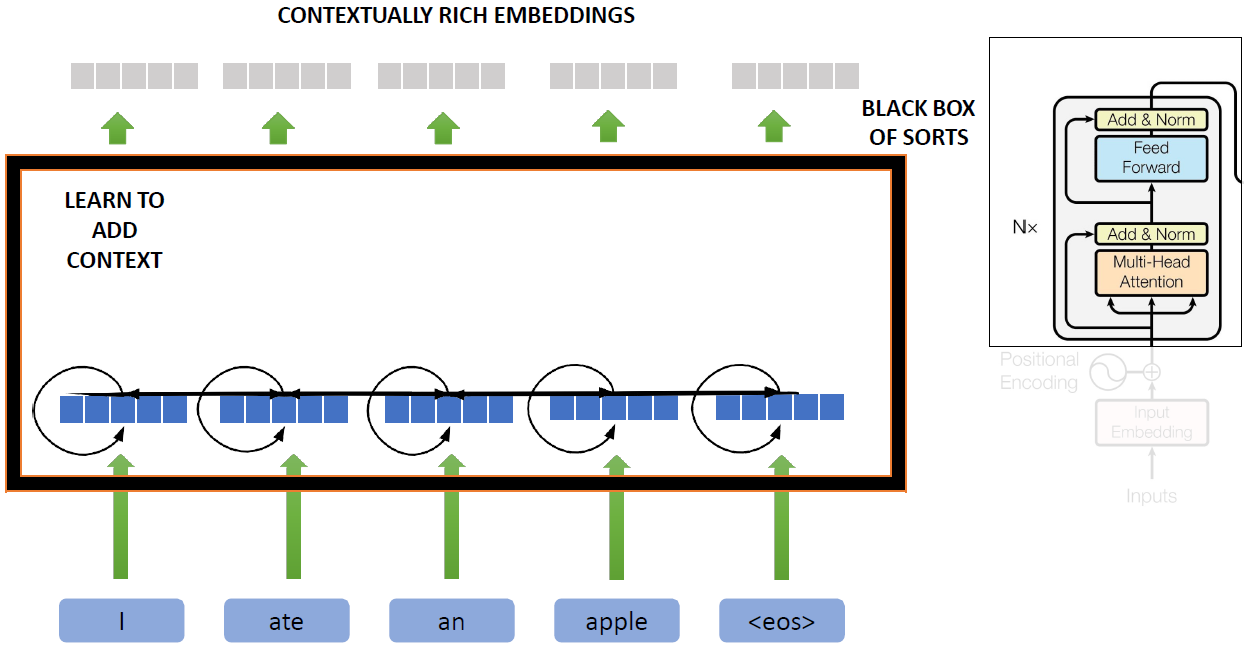
\includegraphics[width=\linewidth, height=0.9\textheight,keepaspectratio]{images/nlp/encoder.png}
    \end{figure}

    \textbf{Encoder} processes the input sequence, generating a set of continuous representations that capture the context and relationships between tokens.
\end{frame}

\begin{frame}{Attention}
    \begin{figure}
        \centering
        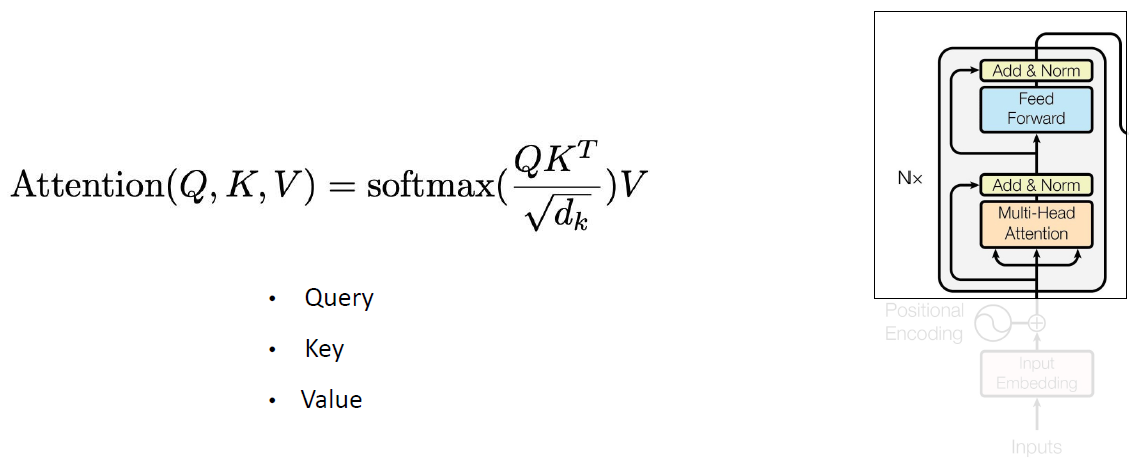
\includegraphics[width=\linewidth, height=0.9\textheight,keepaspectratio]{images/nlp/attention.png}
    \end{figure}
\end{frame}

\begin{frame}[allowframebreaks]{Query, Key, and Value}
    \begin{figure}
        \centering
        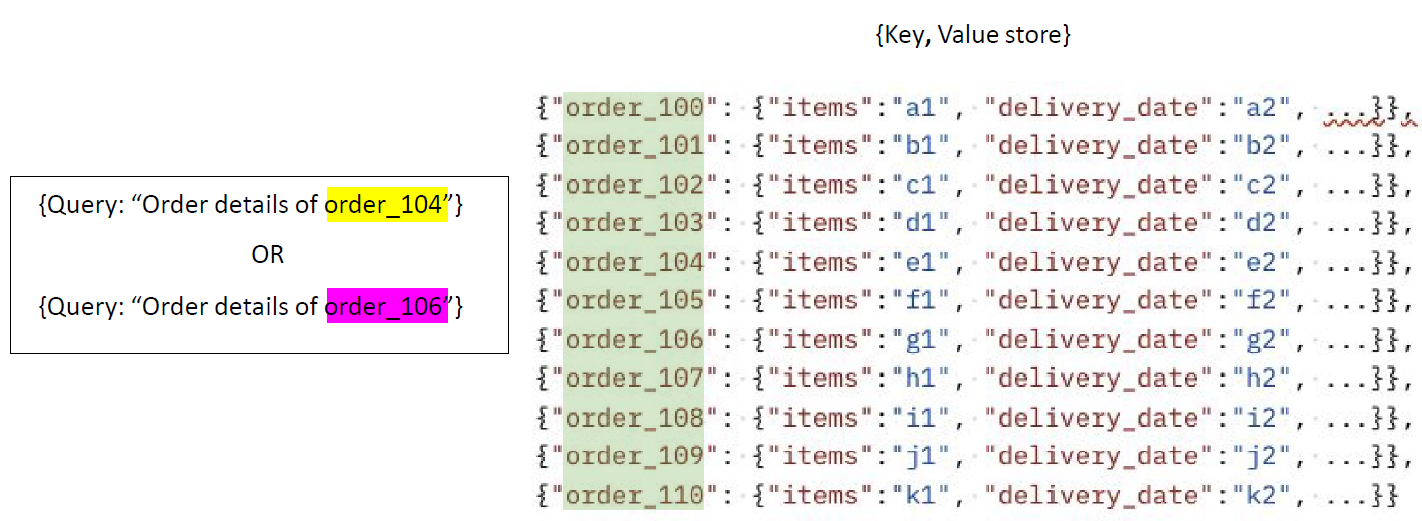
\includegraphics[width=\linewidth, height=0.9\textheight,keepaspectratio]{images/nlp/query-key-value.png}
    \end{figure}

    \framebreak
    \begin{figure}
        \centering
        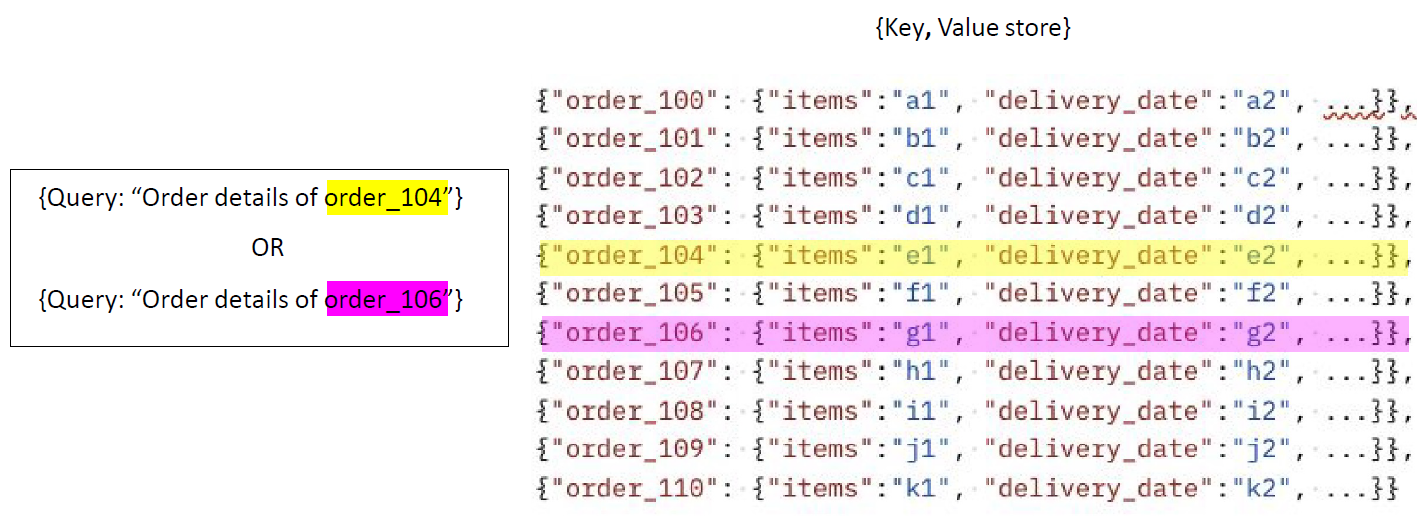
\includegraphics[width=\linewidth, height=0.9\textheight,keepaspectratio]{images/nlp/query-key-value-2.png}
    \end{figure}

    \framebreak
    \begin{figure}
        \centering
        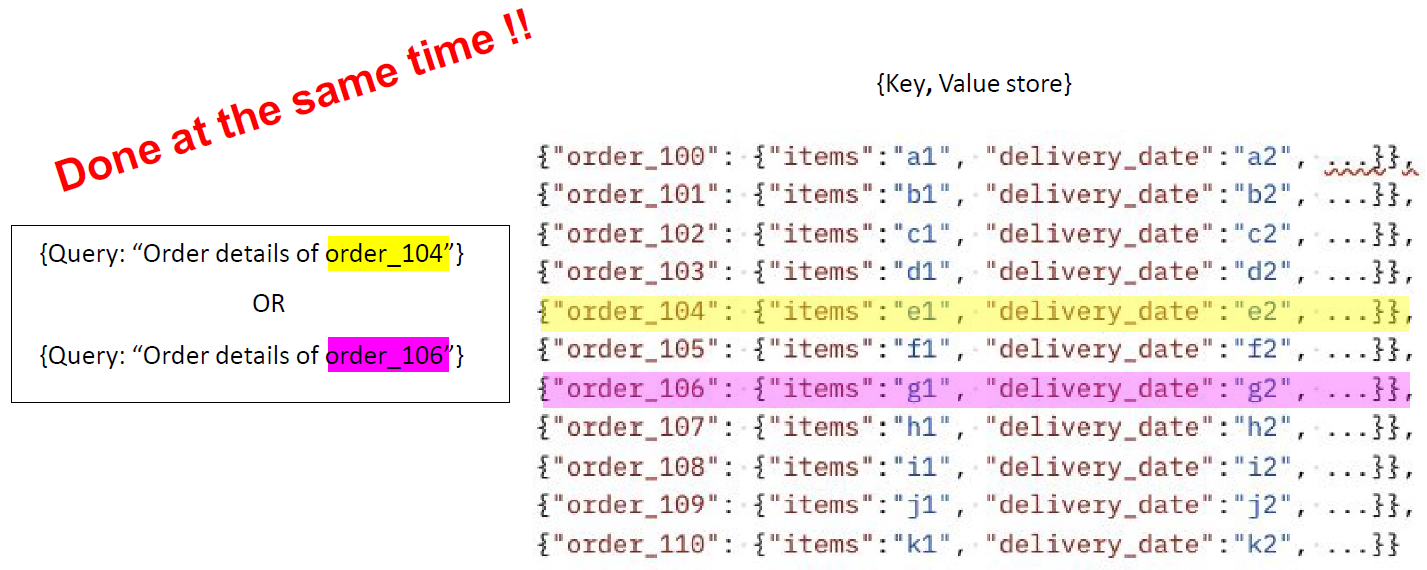
\includegraphics[width=\linewidth, height=0.9\textheight,keepaspectratio]{images/nlp/query-key-value-3.png}
    \end{figure}

    \framebreak
    \begin{figure}
        \centering
        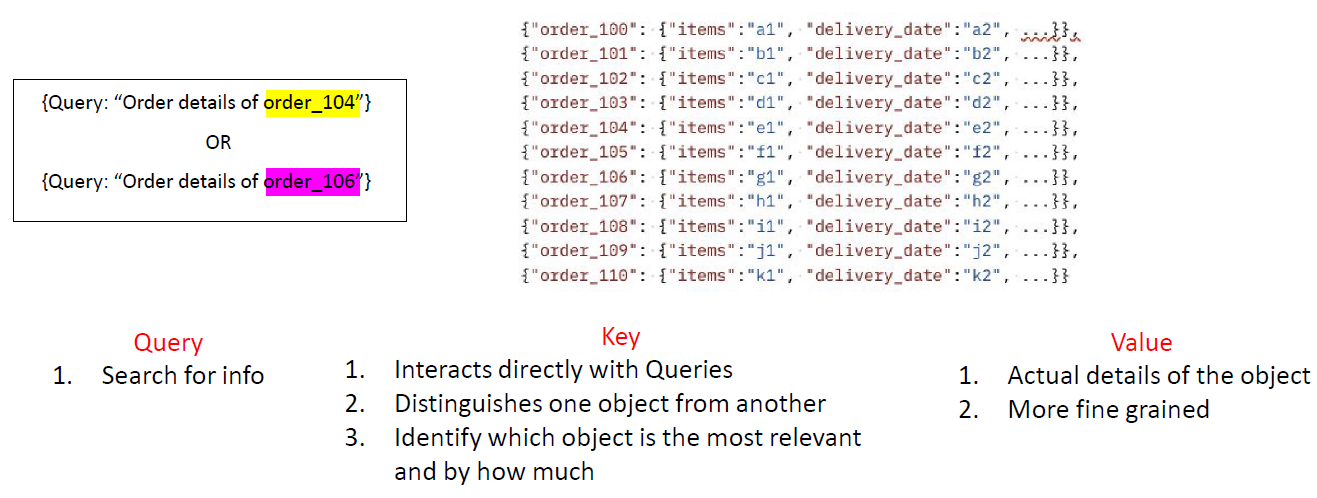
\includegraphics[width=\linewidth, height=0.9\textheight,keepaspectratio]{images/nlp/query-key-value-4.png}
    \end{figure}
\end{frame}

\begin{frame}{Transformers}
    \begin{figure}
        \centering
        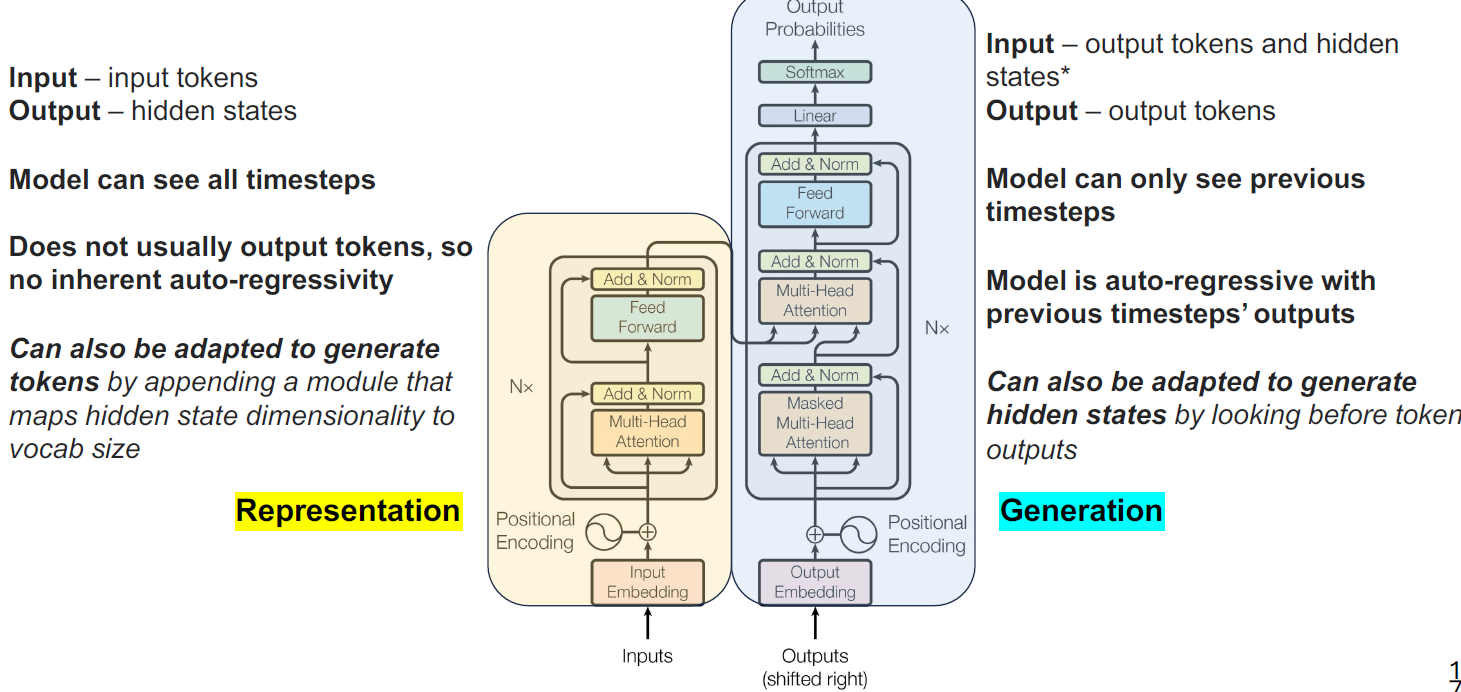
\includegraphics[width=\linewidth, height=0.9\textheight,keepaspectratio]{images/nlp/transformers-architecture-2.png}
    \end{figure}
\end{frame}